\section{Kapitel 1}

\subsection{Symbolisch}

\subsubsection{Allgemein 1. Ordnung}
$\dfrac{d}{dt}y(t)=f(t,y(t)) \qquad y(t_0)=y_0$\\
Eindeutige Lösung $\varphi(t)$ im Intervall falls $f(t,y(t))$ und $\dfrac{d \; f(t,y(t))}{dt}$ stetig im Intervall.
\subsubsection{Linear DGL}
\begin{tabular}{p{6cm}p{2cm}p{10.5cm}}
\textbf{Form:} $y'(t) + p(t) \cdot y(t) = g(t)$ &
\textbf{Vorgehen:}              &

1. $\mu(t)$ berechnen: $\mu(t) = e^{\int p(t) dt}$ \\ &&
2. L"osung: $y(t) = \frac{1}{\mu(t)} \cdot ( \int \mu(t) g(t) dt +c)$ \\ &&
\end{tabular}
Lösung existiert und eindeutig falls $p(t)$ und $g(t)$ stetig.\\
\textbf{Bsp}: $t^3 \cdot y'(t) + 4 t^2 \cdot y(t) = e^{-t} \quad \Longrightarrow \quad y'(t) + \underbrace{4 \frac{1}{t}}_{p(t)} \cdot y(t) = \underbrace{\frac{1}{t^3} e^-t}_{g(t))}$

\subsubsection{Separierbar DGL}
\begin{tabular}{p{6cm}p{2cm}p{10.5cm}}
\textbf{Form:} $M(x) + N(y(x))\cdot y'(x) = 0$ &
\textbf{Vorgehen:}              &

1. $H_1(x)$ berechnen: $H_1(x) = \int M(x) dx$ \\ &&
2. $H_2(y)$ berechnen: $H_2(y) = \int N(y)dy$ \\ &&
3. L"osung: $H_1(x) + H_2(y) = c$ ; c folgt aus Anf. Bed.\\\\
\end{tabular}
\textbf{Bsp}: $y'(x) = (1-2x)y^2 \quad \Longrightarrow \quad \underbrace{-(1-2x)}_{M(x)} + \underbrace{\frac{1}{y^2}}_{N(y(x))} \cdot y'(x) = 0$

\subsubsection{Exakte DGL}
\begin{tabular}{p{6cm}p{2cm}p{10.5cm}}
\textbf{Form:} $M(x,y) + N(x,y)\cdot y'(x) = 0$ &
\textbf{Vorgehen:}              &

1. Kompatibilitaets Bed. pr"ufen: $\diffp{M(x,y)}{y} = \diffp{N(x,y)}{x}$ \\ &&
2. $ M(x,y) = \dfrac{d}{dx}\Psi(x,y) \qquad N(x,y) = \dfrac{d}{dy}\Psi(x,y) $ \\ &&
3. $Q(x,y)$ berechnen: $Q(x,y) = \int M(x,y) dx$ \\ &&
4. $\diffp{h(y)}{y}$ berechnen: $\diffp{h(y)}{y} = N(x,y) - \diffp{Q(x,y)}{y}$ \\ &&
5. $h(y)$ berechnen: $h(y) = \int \diffp{h(y)}{y} dy $ \\ &&
6. L"osung: $\Psi(x,y) = Q(x,y) + h(y) = c $ \\ &&
\end{tabular}
\textbf{Bsp}: $(9x^2 + y -1)dx - (4y -x)dy = 0 \quad \Longrightarrow \quad  \underbrace{9x^2 +y -1}_{M(x,y)} + \underbrace{(-(4y -x))}_{N(x,y)} \cdot \diffp{y}{x} = 0$

\subsection{Nummerisch}
\subsubsection{Fehler}

\begin{tabbing}
Tatzächlicher Wert  \= $\phi(t_n)$ \\
Globaler Fehler \> $E_n = \phi(t_n) - y_n$ \\
Lokaler Fehler \> $e_{n+1} = \phi(t_n + h) - y_{n+1}$ \\
Rundungsfehler \> $R_n = y_n - Y_n$ wobei $Y_n$ gerundet
\end{tabbing}

\subsubsection{Euler}
Polygonzug mit Steigung $y'(t)$\\
$y'(t)=f(t,y(t)) \qquad y(t_0)=y_0 \qquad$ Zeitschritt $h$\\
$t_i = t_{i-1} + h \qquad y_i=y_{i-1} + h \cdot f(t_{i-1},y_{i-1})$\\

$|\phi''(t)|<M \qquad |e_n| < \dfrac{M*h^2}{2} \qquad
h_n < \sqrt{\dfrac{2\epsilon}{M}} \qquad E_n \approx h$\\
$e_{n+1} = \dfrac{1}{2} \cdot \varphi''(\tau_n)\cdot h^2 \qquad \tau_n \text{ zwischenschritt in } [t_n,t_{n+1}]$\\
$\varphi''(t)=f_t(t,\varphi(t)) + f_y(t,\varphi(t))\cdot\varphi'(t)$

\subsubsection{Heun}
Trapez Approximation\\
$y'(t)=f(t,y(t)) \qquad y(t_0)=y_0 \qquad$ Zeitschritt $h$\\
Idee: $y_i=y_{i-1} + h \cdot \dfrac{f(t_{i-1},y_{i-1}) + f(t_{i},y_{i})}{2}$\\
$t_i = t_{i-1} + h \qquad 
y_i = y_{i-1} + h \cdot \dfrac{f(t_{i-1},y_{i-1}) + f(t_{i},y_{i-1} + h \cdot f(t_{i-1},y_{i-1}))}{2}$\\
$e_n \approx h^3 \qquad E_n \approx h^2$
\subsubsection{Runge-Kutta}
$y_{i+1}=y_i + h \cdot \dfrac{k_{i,1} + 2\:k_{i,2} + 2\:k_{i,3} + k_{i,4} }{6}$\\
$k_{i,1} = f(t_{i},y_{i}) \qquad 
k_{i,2} = f(t_{i} + \dfrac{h}{2},y_{i} + \dfrac{h}{2}k_{i,1}) \qquad 
k_{i,3} = f(t_{i} + \dfrac{h}{2},y_{i} + \dfrac{h}{2}k_{i,2}) \qquad 
k_{i,3} = f(t_{i} + h,y_{i} + h \: k_{i,2}) \qquad$\\
$e_n \approx h^5 \qquad E_n \approx h^4$
\subsection{Bifurkationen}
Gegeben ist eine autonome Differentialgleichung mit reellen Parametern.

\begin{equation*}
	\diffp{}{t}y(t) = f(a,y(t))
\end{equation*}

Gesucht die Kritischen punkte die sogenannten Gleichgewichtslösungen. Diese sind wie folgt definiert:
\begin{equation*}
	\diffp{}{t}y(t) = 0
\end{equation*}
Die Gleichgewichtslösungen wird in 3 Fälle unterschieden:\\

\begin{minipage}[h]{0.35\textwidth} 
	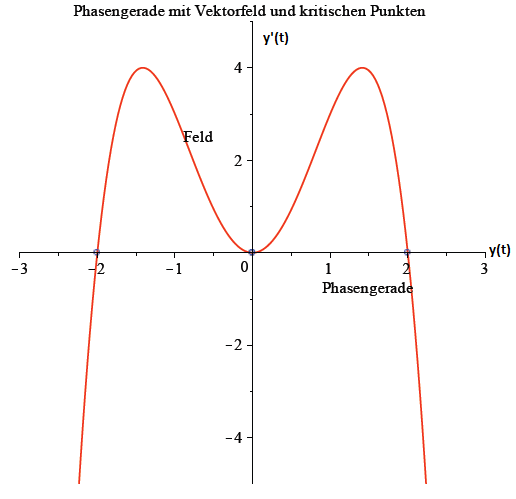
\includegraphics[width=1.0\textwidth]{images/Phasengerade.png}
\end{minipage}
\begin{minipage}[h]{0.35\textwidth}
	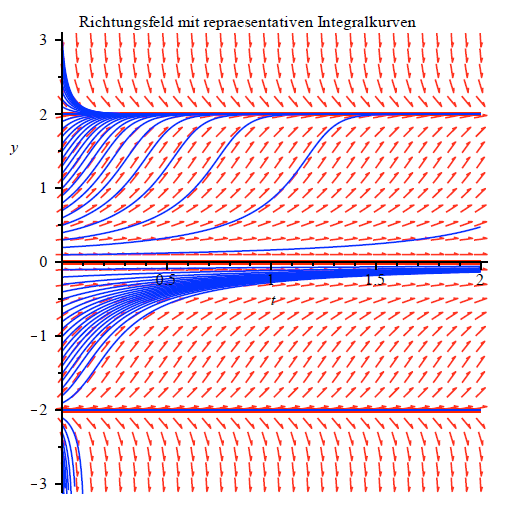
\includegraphics[width=1.0\textwidth]{images/Richtungsfeld.png}
\end{minipage}
\begin{tabular}{p{1.8cm}p{5cm}}
	$y(t) = -2$: & instabiel \\
	$y(t) = 0$: & semistabil\\
	$y(t) = 2$: & asymtotisch stabil\\
\end{tabular}

\subsection{Bifurkationsdiagramm}
\begin{minipage}[h]{0.35\textwidth}
$y'=y(a-y)$\\
Kritische Punkte in Abhängikeit von $a$\\
\begin{tabbing}
Ausgezogen: \= Asymptotisch Stabil\\
Gestrichelt: \> Instabil\\
Zentrum: \> Semistabil\\
\end{tabbing}
\end{minipage}
\begin{minipage}[h]{0.35\textwidth}
	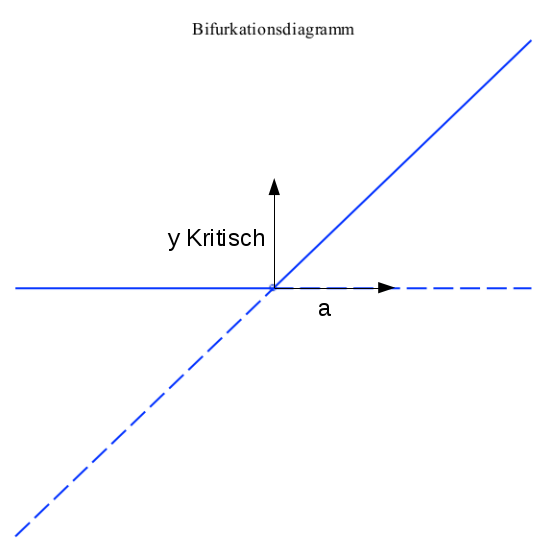
\includegraphics[width=1.0\textwidth]{images/Bifurkationsdiagramm.png}
\end{minipage}